\chapter{Results and Future Work}
\label{capitolo8}
\thispagestyle{empty}
\section{Results}
After this long jurney through solar physics and deep learning, we finally arrived to the results. But before considering the performance of the algorithm, let's have a closer look at the dataset that will be used as a baseline. Among all the sources that provide an estimation of the superficial activity of the Sun using white-light data, the International Sunspot Number (ISN), provided by SIDC-SILSO, is certainly the most used. Its popularity is due to the fact that it try to conjugate traditional observation techniques with modern standards of accuracy. This is achieved by using a network of stations composed by professionals and amateurs, located all around the world, although mostly in Europe. Also, what is interesting for us is that all annotations are done manually, directly from the eyepiece of the telescope or projecting the light on a white plate and then drawing on top of it.
\bigbreak
\noindent Behind these choices there is the strong convinction that modern technology is, in some sense, still too limited and human supervision is required for robust estimations. This work proposes the idea that deep learning, being able to learn from human-produced experience, could be the tool that changes this trend. To demostrate this point we need to be able to compare the results of our solution to the ones obtained by humans. Luckily, SIDC-SILSO includes in the dataset the value of the standard deviation as well as the number of data points included in the calculation (number of stations). This, besides allowing the assessment the precision of the value, enables us to compare the expected error of humans with ours.
\bigbreak
\noindent The final results that will be shown in this chapter are all computed on the test set (containing both ground-based and space-based observations) and employ the parameters that where estimated on the validation set. For the prediction of the sunspot number on the test images, the procedure explaied in section \ref{autoannotation} is used. Then, day by day, the detected number of sunspots is compared to the one found in the dataset, and the error is computed. To help visualization, the final value and the error are averaged monthly for both our results and the baseline. Although monthly smoothing works well to get an idea of the behaviour of the algorithm, we remind the reader that the average is computed only on the days that belong to the test set, and therefore it does not represent a good indicator of the overall trend of the solar cycle.
\bigbreak
\begin{figure}[t!]
  \centering
  \captionsetup{justification=centering}
  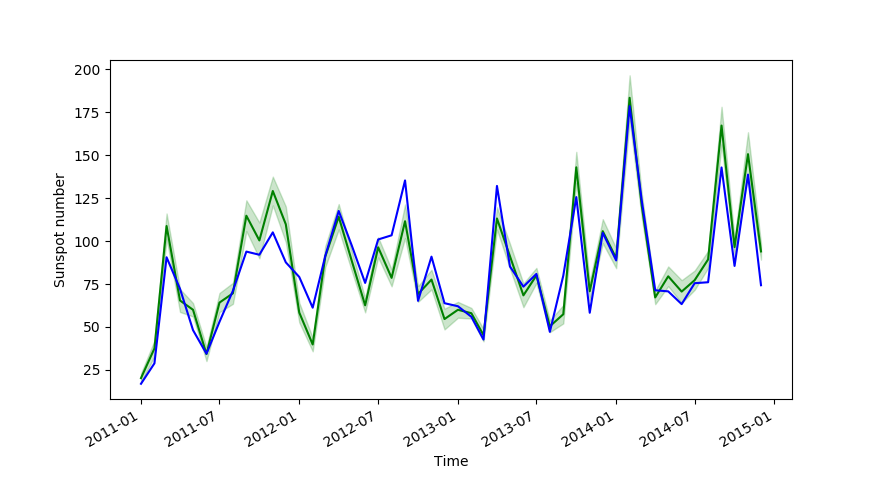
\includegraphics[width=\textwidth]{./pictures/result-monthly-3}
  \caption{Comparison between monthly averages of our algorithm (blue) and the international sunspot number (green) with confidence interval.}
  \label{fig:result-monthly-3}
\end{figure}
\noindent Figure~\ref{fig:result-monthly-3} shows the sunspot number derived with the relative sunspot formula as calculated by our algorithm (blue) compared to the ISN provided by SIDC-SILSO. The plot also shows the confidence interval (standard deviation) for the ISN measurement. The algorithm seems to have learned to identify the tendency of the activity, in fact, the two lines follow roughly the same trend. Although, a closer inspection reveals that, in general, the deviation from the ISN is not neglectable.
\bigbreak
\noindent Comparing the error generated by our algorithm and the standard error of the ISN (Figure~\ref{fig:error-norm}), we discover that there is no strong evidence of correlation between the two errors. This means that the reasons why humans make mistakes are probably not the same as the ones that make our algorithm fail. Anyhow, the error produced by our solution seems to be larger than the average human error. Summing up all the errors together over the whole test set, it turns out that the average errors are:
\begin{itemize}
  \item around 13 units (18\%) for our algorithm;
  \item around 6 units (8\%) for the the average station in the ISN network.
\end{itemize}
\bigbreak
\noindent Since the SIDC-SILSO receives the pre-computed sunspot number from the station of the network, they do not need to calculate the number of groups and therefore they do not provide it in the data. This makes it a lot harder to understand the causes of the misalignment between the two measurements. Anyway we can make pretty confident hypotheses on why this happens. The first reason is related to the annotation method. In fact, the data (DPD dataset) provided to the algorithm for training and validation is annotated a posteriori from images of the disk, while the stations of the SIDC-SILSO network make live observations looking at the Sun. This problem is really difficult to overcome, because live observations are hard to turn into a digital format automatically and create a dataset with them.
\bigbreak
\begin{figure}[t!]
  \centering
  \captionsetup{justification=centering}
  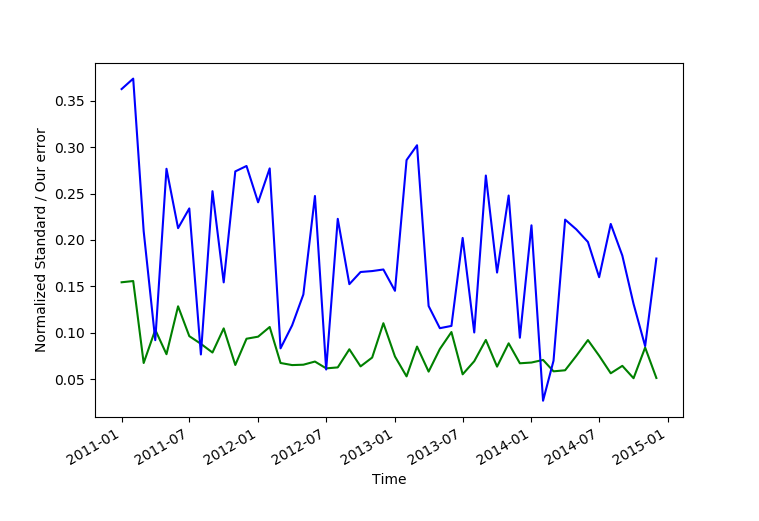
\includegraphics[width=\textwidth]{./pictures/error-norm}
  \caption{Comparison between normalized ISN standard error (green) and the normalized error of our algorithm (blue)}
  \label{fig:error-norm}
\end{figure}
\noindent Another solid reason for the deviation in the estimation of the sunspot number has its roots in the types of observatories that are used. On the one hand, we rely on the best observatories that are available, which are able to detect even small pores on the surface of the Sun. On the other hand, two thirds of the observatories of the SIDC-SILSO network use amatorial instrumentations that are not able to resolve all the sunspots on the disk. This hypotheses is also supported by the fact that the personal reduction coefficient of our algorithm is very low, meaning that it is able to detect a large amount of sunspots.
\bigbreak
\noindent Nonetheless, despite the marginal problems that have been identified, we succeded in the creation of an algorithm that can capture the fluctuations in the sunspot count and therefore it can be used to predict the activity of our star. As the title of this thesis suggests, this is an initial deep learning approach to the problem, thus we hope that many more similar algorithms will be explored in the future, building upon ours and increasing its performance.
\section{Future Work}
The procedure described in this thesis can be considered complete, in the sense that we proposed a solution that works from the beginning to the end without overlooking intermediate steps. Although this, there is still a lot of work to do in order to make the algorithm ready to be used for scientific purposes reliably.
\bigbreak
\noindent Certainly, the part that needs most revision is the data. In fact, although the Decebren database (DPD) is a great place to start because it provides detailed annotations, the quantity of data could be increased. So far, only the peak years of the solar cycle 24 have been used to train the models, previous cycles should be added to increase the variablity of the data. The deep learning models that were used would undoubtedly benefit from a wider set of examples to draw knowledge. From the work, we also learned that the annotations of the images should depend on the scope of application, so they need to be selected accordingly.
\bigbreak
\noindent Another aspect that should be explored better is the minimization of dependencies among training, validation and test set. Even though we took them into account in the process of splitting of the dataset, we didn't succeed in removing them completely. For the splitting to be independent, it would be required to check if each sunspot group appears in only one of the three chunks of data. Removing the images where the groups are repeated is always possile, at the cost of sensibly reducing the size of the dataset. Another approach is to use an algorithm that minimizes the groups that belong to the overlapping of the three sets. Since brute-forcing over thousands of groups is out of question, genetic algorithms may be used to find suboptimal solutions.
\bigbreak
\noindent For what concerns the final results, more test cases can be designed. The comparison with the international sunspot number produced contrasting results. To clarify the situation, it is possible to analyze the deviation of our sunspot number with other datasets. For example, the american National Oceanic and Atmospheric Administration (NOAA) produces a similar time series, whose properties are, though, a bit different from the ISN. Besides that, other indicators can be analyzed. For instance, it is not unusual for the scientists to refer to the ``backbone'' number of groups for some studies, or even simply to the total area of sunspots on the disk. It is unclear which one of these measures is most suited as a base for more complex studies, but that is actually out of the scope of this work. It is sufficient for us to be able to compare our results with some human-produced ones. The drawback of these other datasets, that is also the reason why ISN was selected, is that they lack the measure of standard deviation because they are not computed ensembling human measurements.
\bigbreak
\noindent On the other hand, for what concerns more structural and algorithmical aspects, even though our framework seems well established, some minor modifications can be made. For instance, the triplet loss can be used instead of the contrastive one for the training of the siamese network, to see if it improves the performance. The segmentation as well may be improved by moving the discovery of the umbra inside the U-Net. This can be achieved assigning different classes for umbra and penumbra, and then optimizing the network for the new multi-class problem. A dramatically different approach, instead, would be to perform the clustering phase inside the U-Net, together with semantic segmentation. This is called instance segmentation and it is known to be very hard to train, hence why it has been discarded in this work. The great advantage of being able to recognize instances would be the simplification of the workflow, since only one network would be evaluated to get both the number of clusters and single sunspots.
\bigbreak
\noindent Some of these solutions will probably be explored in the future in the hope of improving this tool and making it publicly available online for scientific and eduactional purposes.
